\documentclass[10pt,twocolumn]{article}
\usepackage{graphicx}
\usepackage[margin=0.5in]{geometry}
\usepackage[cmex10]{amsmath}
\usepackage{array}
\usepackage{booktabs}
\usepackage{mathtools}
\title{\textbf{Optimization Assignment - 2}}
\author{Thoutu Rahul Raj}

\providecommand{\norm}[1]{\lVert#1\rVert}
\providecommand{\abs}[1]{\vert#1\vert}
\let\vec\mathbf
\newcommand{\myvec}[1]{\ensuremath{\begin{pmatrix}#1\end{pmatrix}}}
\newcommand{\mydet}[1]{\ensuremath{\begin{vmatrix}#1\end{vmatrix}}}
\providecommand{\brak}[1]{\ensuremath{\left(#1\right)}}
\providecommand{\lbrak}[1]{\ensuremath{\left(#1\right.}}
\providecommand{\rbrak}[1]{\ensuremath{\left.#1\right)}}
\providecommand{\sbrak}[1]{\ensuremath{{}\left[#1\right]}}

\begin{document}

\maketitle
\paragraph{\textit{Problem Statement} - Find the maximum isosceles triangle inscribable in a given ellipse,i.e,find the maximum value of xy,having given\\
\large{$ \frac{x^2}{a^2}$+$\frac{y^2}{b^2}$=1.}
\begin{align*}
f(x) = absin\theta(1-cos\theta)
\end{align*}} 

\section{Solution}
\begin{flushleft}
Given function is,\\
\end{flushleft}
\begin{equation}
    f(x)=absin\theta(1-cos\theta)
\end{equation}
\subsection{Calculation using normal differentiation}
\begin{flushleft}
Differentiating (1) yields,
\end{flushleft}
\begin{align}
\nabla f(x) = ab(cos\theta-cos2\theta)
\end{align}

\noindent Calculating the critical points:
$ \nabla f(x) = 0 $

\begin{equation}
\implies \cos{x} = 0 
\end{equation}
\begin{equation}
\implies cos2\theta = 0
\end{equation}
Therefore, the critical points are 

\begin{equation}
{\pi}n,\quad\frac{\pi}{2}+n\pi
\end{equation}
Hence, 
\begin{align}
\text{absolute maximum} & =  1.9999\\
\end{align}

\subsection{Calculation of Maxima using gradient ascent algorithm}
$f(x) = absin\theta(1-cos\theta)$\\
\begin{align}
\max_{x} f(x)
\end{align} 
Maxima of eq(1) is calculated by using gradient ascent method
\begin{align}
x_{n+1} = x_n + \alpha \nabla f(x_n) 
\end{align}
\begin{align}
x_{n+1} &= x_n + \alpha \brak{cosx_n-2sinx_ncosx_n}
\end{align}
where \\
1)$x_0=0.5$ \\
2)$\alpha=0.001$ \\
3)precision $= 0.00000001$ \\
values obtained using python are:
    \begin{align}
        \boxed{\text{Maxima} = 1.999 }\\
        \boxed{\text{Maxima Point} = 0.7853}
    \end{align}
    
\begin{figure}[h!]
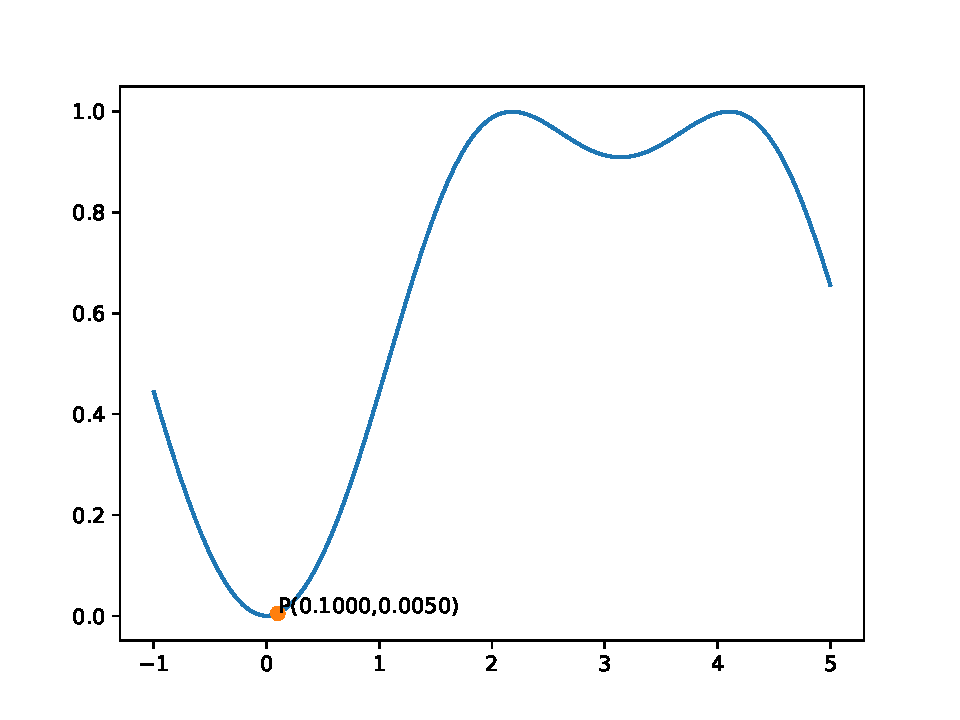
\includegraphics[scale=0.55]{opt2.pdf}
\caption{The function f(x) with maxima and minima points}
\end{figure}        
\end{document}
